% Created by tikzDevice version 0.12.6 on 2026-09-22 18:57:08
% !TEX encoding = UTF-8 Unicode
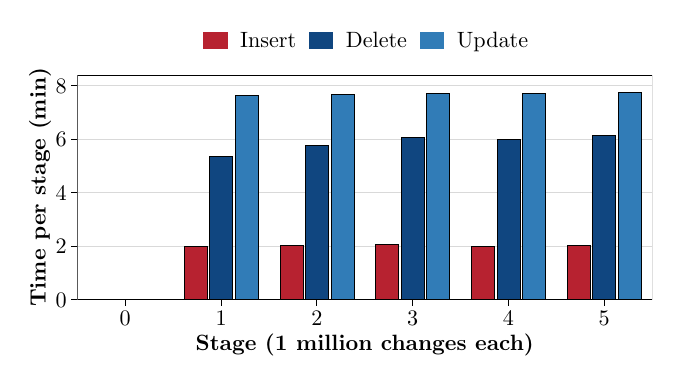
\begin{tikzpicture}[x=1pt,y=1pt]
\definecolor{fillColor}{RGB}{255,255,255}
\path[use as bounding box,fill=fillColor,fill opacity=0.00] (0,0) rectangle (227.65,119.25);
\begin{scope}
\path[clip] (  0.00,  0.00) rectangle (227.65,119.25);
\definecolor{fillColor}{RGB}{255,255,255}

\path[fill=fillColor] (  0.00,  0.00) rectangle (227.65,119.25);
\end{scope}
\begin{scope}
\path[clip] ( 17.95, 21.02) rectangle (225.65,102.13);
\definecolor{fillColor}{RGB}{255,255,255}

\path[fill=fillColor] ( 17.95, 21.02) rectangle (225.65,102.13);
\definecolor{drawColor}{gray}{0.85}

\path[draw=drawColor,line width= 0.3pt,line join=round] ( 17.95, 21.02) --
	(225.65, 21.02);

\path[draw=drawColor,line width= 0.3pt,line join=round] ( 17.95, 40.33) --
	(225.65, 40.33);

\path[draw=drawColor,line width= 0.3pt,line join=round] ( 17.95, 59.64) --
	(225.65, 59.64);

\path[draw=drawColor,line width= 0.3pt,line join=round] ( 17.95, 78.96) --
	(225.65, 78.96);

\path[draw=drawColor,line width= 0.3pt,line join=round] ( 17.95, 98.27) --
	(225.65, 98.27);
\definecolor{fillColor}{RGB}{183,34,48}

\path[fill=fillColor] ( 56.49, 21.02) rectangle ( 64.80, 40.20);

\path[fill=fillColor] ( 91.11, 21.02) rectangle ( 99.42, 40.45);

\path[fill=fillColor] (125.72, 21.02) rectangle (134.03, 40.88);

\path[fill=fillColor] (160.34, 21.02) rectangle (168.65, 40.27);

\path[fill=fillColor] (194.96, 21.02) rectangle (203.27, 40.47);
\definecolor{fillColor}{RGB}{16,70,128}

\path[fill=fillColor] ( 65.72, 21.02) rectangle ( 74.03, 72.69);

\path[fill=fillColor] (100.34, 21.02) rectangle (108.65, 76.69);

\path[fill=fillColor] (134.96, 21.02) rectangle (143.26, 79.78);

\path[fill=fillColor] (169.57, 21.02) rectangle (177.88, 78.95);

\path[fill=fillColor] (204.19, 21.02) rectangle (212.50, 80.20);
\definecolor{fillColor}{RGB}{49,124,183}

\path[fill=fillColor] ( 74.95, 21.02) rectangle ( 83.26, 94.84);

\path[fill=fillColor] (109.57, 21.02) rectangle (117.88, 95.05);

\path[fill=fillColor] (144.19, 21.02) rectangle (152.49, 95.47);

\path[fill=fillColor] (178.80, 21.02) rectangle (187.11, 95.70);

\path[fill=fillColor] (213.42, 21.02) rectangle (221.73, 95.97);
\definecolor{drawColor}{RGB}{0,0,0}

\path[draw=drawColor,line width= 0.2pt] ( 56.49, 21.02) rectangle ( 64.80, 40.20);

\path[draw=drawColor,line width= 0.2pt] ( 91.11, 21.02) rectangle ( 99.42, 40.45);

\path[draw=drawColor,line width= 0.2pt] (125.72, 21.02) rectangle (134.03, 40.88);

\path[draw=drawColor,line width= 0.2pt] (160.34, 21.02) rectangle (168.65, 40.27);

\path[draw=drawColor,line width= 0.2pt] (194.96, 21.02) rectangle (203.27, 40.47);

\path[draw=drawColor,line width= 0.2pt] ( 65.72, 21.02) rectangle ( 74.03, 72.69);

\path[draw=drawColor,line width= 0.2pt] (100.34, 21.02) rectangle (108.65, 76.69);

\path[draw=drawColor,line width= 0.2pt] (134.96, 21.02) rectangle (143.26, 79.78);

\path[draw=drawColor,line width= 0.2pt] (169.57, 21.02) rectangle (177.88, 78.95);

\path[draw=drawColor,line width= 0.2pt] (204.19, 21.02) rectangle (212.50, 80.20);

\path[draw=drawColor,line width= 0.2pt] ( 74.95, 21.02) rectangle ( 83.26, 94.84);

\path[draw=drawColor,line width= 0.2pt] (109.57, 21.02) rectangle (117.88, 95.05);

\path[draw=drawColor,line width= 0.2pt] (144.19, 21.02) rectangle (152.49, 95.47);

\path[draw=drawColor,line width= 0.2pt] (178.80, 21.02) rectangle (187.11, 95.70);

\path[draw=drawColor,line width= 0.2pt] (213.42, 21.02) rectangle (221.73, 95.97);

\path[draw=drawColor,line width= 0.4pt,line join=round,line cap=round] ( 17.95, 21.02) rectangle (225.65,102.13);
\end{scope}
\begin{scope}
\path[clip] (  0.00,  0.00) rectangle (227.65,119.25);
\definecolor{drawColor}{RGB}{0,0,0}

\node[text=drawColor,anchor=base east,inner sep=0pt, outer sep=0pt, scale=  0.80] at ( 14.08, 18.26) {0};

\node[text=drawColor,anchor=base east,inner sep=0pt, outer sep=0pt, scale=  0.80] at ( 14.08, 37.58) {2};

\node[text=drawColor,anchor=base east,inner sep=0pt, outer sep=0pt, scale=  0.80] at ( 14.08, 56.89) {4};

\node[text=drawColor,anchor=base east,inner sep=0pt, outer sep=0pt, scale=  0.80] at ( 14.08, 76.20) {6};

\node[text=drawColor,anchor=base east,inner sep=0pt, outer sep=0pt, scale=  0.80] at ( 14.08, 95.51) {8};
\end{scope}
\begin{scope}
\path[clip] (  0.00,  0.00) rectangle (227.65,119.25);
\definecolor{drawColor}{RGB}{0,0,0}

\path[draw=drawColor,line width= 0.3pt,line join=round] ( 15.68, 21.02) --
	( 17.95, 21.02);

\path[draw=drawColor,line width= 0.3pt,line join=round] ( 15.68, 40.33) --
	( 17.95, 40.33);

\path[draw=drawColor,line width= 0.3pt,line join=round] ( 15.68, 59.64) --
	( 17.95, 59.64);

\path[draw=drawColor,line width= 0.3pt,line join=round] ( 15.68, 78.96) --
	( 17.95, 78.96);

\path[draw=drawColor,line width= 0.3pt,line join=round] ( 15.68, 98.27) --
	( 17.95, 98.27);
\end{scope}
\begin{scope}
\path[clip] (  0.00,  0.00) rectangle (227.65,119.25);
\definecolor{drawColor}{RGB}{0,0,0}

\path[draw=drawColor,line width= 0.3pt,line join=round] ( 35.26, 18.74) --
	( 35.26, 21.02);

\path[draw=drawColor,line width= 0.3pt,line join=round] ( 69.88, 18.74) --
	( 69.88, 21.02);

\path[draw=drawColor,line width= 0.3pt,line join=round] (104.49, 18.74) --
	(104.49, 21.02);

\path[draw=drawColor,line width= 0.3pt,line join=round] (139.11, 18.74) --
	(139.11, 21.02);

\path[draw=drawColor,line width= 0.3pt,line join=round] (173.73, 18.74) --
	(173.73, 21.02);

\path[draw=drawColor,line width= 0.3pt,line join=round] (208.34, 18.74) --
	(208.34, 21.02);
\end{scope}
\begin{scope}
\path[clip] (  0.00,  0.00) rectangle (227.65,119.25);
\definecolor{drawColor}{RGB}{0,0,0}

\node[text=drawColor,anchor=base,inner sep=0pt, outer sep=0pt, scale=  0.80] at ( 35.26, 11.63) {0};

\node[text=drawColor,anchor=base,inner sep=0pt, outer sep=0pt, scale=  0.80] at ( 69.88, 11.63) {1};

\node[text=drawColor,anchor=base,inner sep=0pt, outer sep=0pt, scale=  0.80] at (104.49, 11.63) {2};

\node[text=drawColor,anchor=base,inner sep=0pt, outer sep=0pt, scale=  0.80] at (139.11, 11.63) {3};

\node[text=drawColor,anchor=base,inner sep=0pt, outer sep=0pt, scale=  0.80] at (173.73, 11.63) {4};

\node[text=drawColor,anchor=base,inner sep=0pt, outer sep=0pt, scale=  0.80] at (208.34, 11.63) {5};
\end{scope}
\begin{scope}
\path[clip] (  0.00,  0.00) rectangle (227.65,119.25);
\definecolor{drawColor}{RGB}{0,0,0}

\node[text=drawColor,anchor=base,inner sep=0pt, outer sep=0pt, scale=  0.80] at (121.80,  2.56) {\bfseries Stage (1 million changes each)};
\end{scope}
\begin{scope}
\path[clip] (  0.00,  0.00) rectangle (227.65,119.25);
\definecolor{drawColor}{RGB}{0,0,0}

\node[text=drawColor,rotate= 90.00,anchor=base,inner sep=0pt, outer sep=0pt, scale=  0.80] at (  6.52, 61.57) {\bfseries Time per stage (min)};
\end{scope}
\begin{scope}
\path[clip] (  0.00,  0.00) rectangle (227.65,119.25);
\definecolor{fillColor}{RGB}{255,255,255}

\path[fill=fillColor] ( 62.78,110.13) rectangle (180.82,118.25);
\end{scope}
\begin{scope}
\path[clip] (  0.00,  0.00) rectangle (227.65,119.25);
\definecolor{fillColor}{RGB}{183,34,48}

\path[fill=fillColor] ( 63.30,111.65) rectangle ( 72.22,117.73);
\end{scope}
\begin{scope}
\path[clip] (  0.00,  0.00) rectangle (227.65,119.25);
\definecolor{fillColor}{RGB}{16,70,128}

\path[fill=fillColor] (101.54,111.65) rectangle (110.47,117.73);
\end{scope}
\begin{scope}
\path[clip] (  0.00,  0.00) rectangle (227.65,119.25);
\definecolor{fillColor}{RGB}{49,124,183}

\path[fill=fillColor] (141.61,111.65) rectangle (150.53,117.73);
\end{scope}
\begin{scope}
\path[clip] (  0.00,  0.00) rectangle (227.65,119.25);
\definecolor{drawColor}{RGB}{0,0,0}

\node[text=drawColor,anchor=base west,inner sep=0pt, outer sep=0pt, scale=  0.80] at ( 76.74,111.93) {Insert};
\end{scope}
\begin{scope}
\path[clip] (  0.00,  0.00) rectangle (227.65,119.25);
\definecolor{drawColor}{RGB}{0,0,0}

\node[text=drawColor,anchor=base west,inner sep=0pt, outer sep=0pt, scale=  0.80] at (114.98,111.93) {Delete};
\end{scope}
\begin{scope}
\path[clip] (  0.00,  0.00) rectangle (227.65,119.25);
\definecolor{drawColor}{RGB}{0,0,0}

\node[text=drawColor,anchor=base west,inner sep=0pt, outer sep=0pt, scale=  0.80] at (155.05,111.93) {Update};
\end{scope}
\end{tikzpicture}
